\documentclass[10pt]{article}

\usepackage[utf8]{inputenc}
\usepackage[T2A]{fontenc}
\usepackage[russian, english]{babel}

\usepackage{amssymb, amsmath, textcomp, tabularx, graphicx}
\usepackage{indentfirst}
\usepackage{listings}

\title{Отчет по заданию 3}
\author{Андрей Коновалов, 073}
\date{}

\begin{document}

\maketitle

\section{Постановка задачи}

Для 103 образцов раствора бетона известно содержание в кубическом метре семи основных компонент, для каждого образца измерены также осадка, растекание и прочность на сжатие.
Хочется построить функцию, оценивающую растекание бетона по его составу.

\section{Построение модели}

Визуализация исходных данных приведена на рис. 1.
На рис. 2 приведена гистограмма растеканий, по которой видно, что выбросов по растеканиям нет.
Поскольку $\frac{\max y}{\min y} = 4$, то преобразование растекания искать нецелесообразно.

\begin{figure}[h]
  \centering
  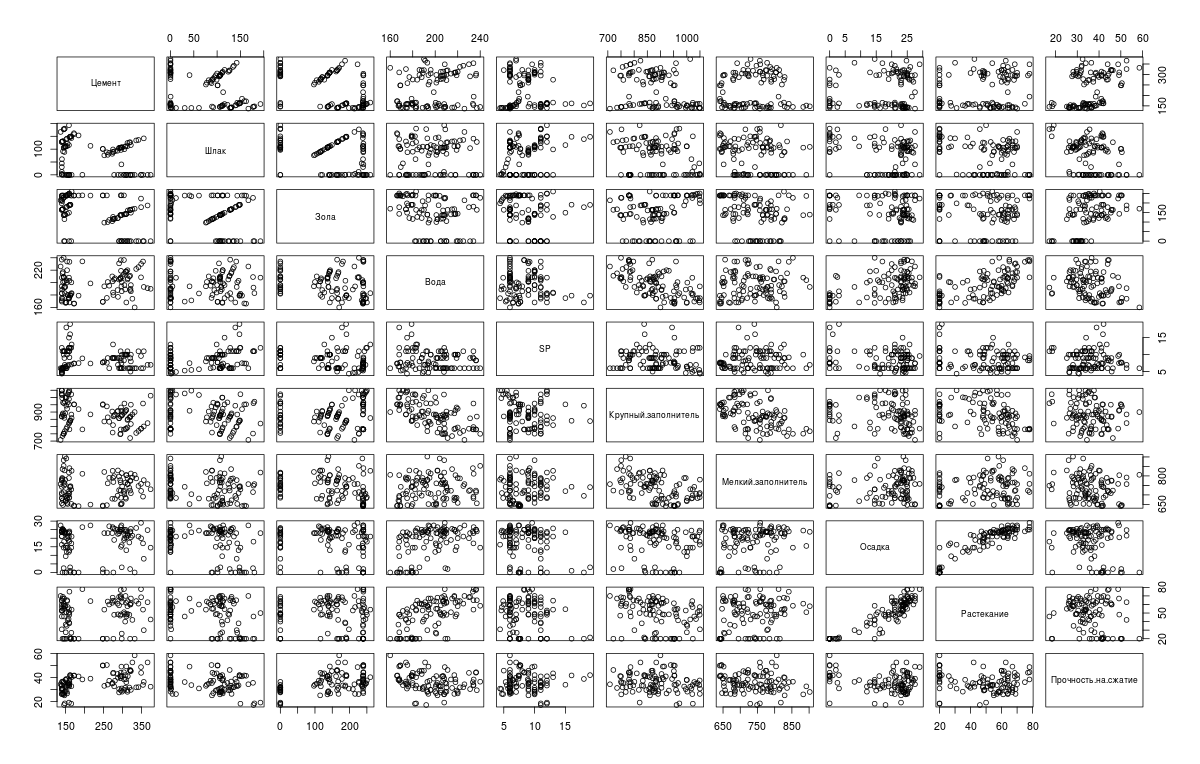
\includegraphics[scale=0.33]{visualization.png}
  \caption{Визуализация данных.}
\end{figure}

\begin{figure}[h]
  \centering
  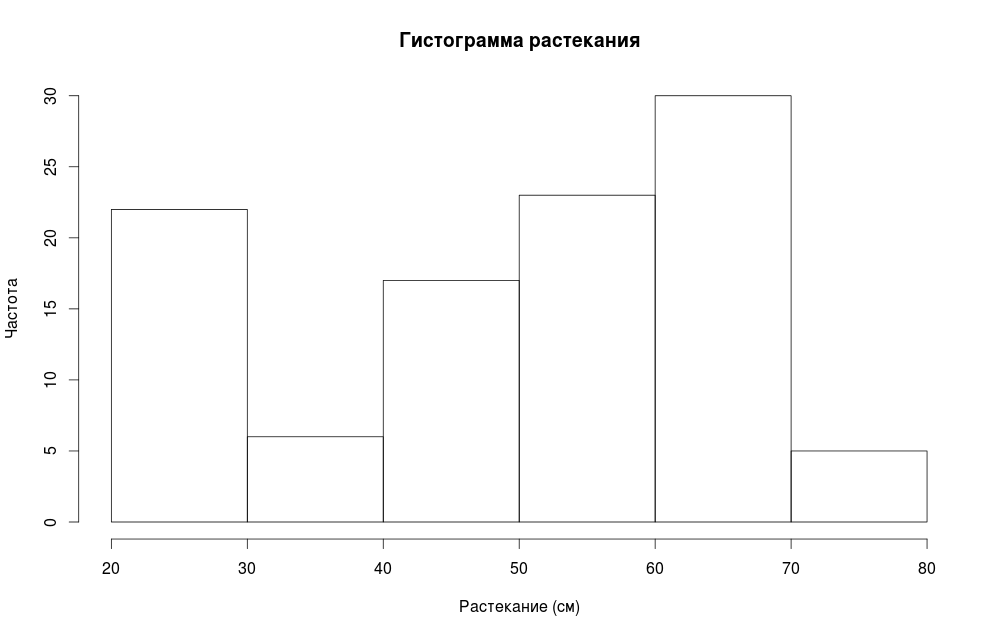
\includegraphics[scale=0.4]{hist.png}
  \caption{Гистограмма растекания.}
\end{figure}

\subsection{Модель 1}

Построим линейную модель 1 с учетом всех факторов:

\begin{verbatim}
> fit1 <- lm(formula = Растекание ~ Цемент + Шлак + Зола + Вода +
  SP + Крупный.заполнитель + Мелкий.заполнитель, data = data)
> summary(fit1)

Call:
lm(formula = Растекание ~ Цемент + Шлак + 
    Зола + Вода + SP + Крупный.заполнитель + 
    Мелкий.заполнитель, data = data)

Residuals:
    Min      1Q  Median      3Q     Max 
-30.880 -10.428   1.815   9.601  22.953 

Coefficients:
                      Estimate Std. Error t value Pr(>|t|)  
(Intercept)         -252.87467  350.06649  -0.722   0.4718  
Цемент                 0.05364    0.11236   0.477   0.6342  
Шлак                  -0.00569    0.15638  -0.036   0.9710  
Зола                   0.06115    0.11402   0.536   0.5930  
Вода                   0.73180    0.35282   2.074   0.0408 *
SP                     0.29833    0.66263   0.450   0.6536  
Крупный.заполнитель    0.07366    0.13510   0.545   0.5869  
Мелкий.заполнитель     0.09402    0.14191   0.663   0.5092  
---
Signif. codes:  0 ‘***’ 0.001 ‘**’ 0.01 ‘*’ 0.05 ‘.’ 0.1 ‘ ’ 1

Residual standard error: 12.84 on 95 degrees of freedom
Multiple R-squared:  0.5022,	Adjusted R-squared:  0.4656 
F-statistic: 13.69 on 7 and 95 DF,  p-value: 3.915e-12
\end{verbatim}

У полученной модели:
$$
  R^2 = 0.5022, \; R^2_{\alpha} = 0.4656, \; F = 13.69, \; \text{p-value} = 3.915 \cdot 10^{-12}
$$

Проверим нормальность, несмещенность и гомоскедастичность:

\bigskip

\begin{tabularx}{\textwidth}{ |X|c| }
  \hline
  Критерий & p-value \\
  \hline
  Шапиро-Уилка (нормальность) & 0.0428 \\
  \hline
  Уилкоксона (несмещенность) & 0.7987 \\
  \hline
  Бройша-Пагана (гомоскедастичность) & 0.09443 \\
  \hline
\end{tabularx}

\bigskip

На рис. 3 приведены нормализованные остатки для полученной модели.
По графику видно, что больших выбросов нет.

\begin{figure}[h]
  \centering
  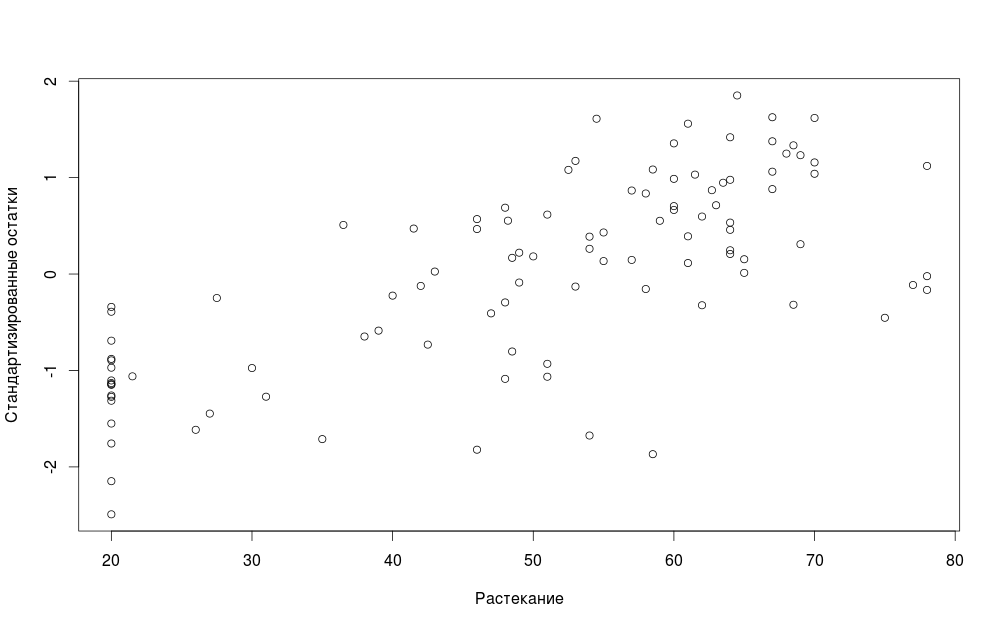
\includegraphics[scale=0.4]{standres.png}
  \caption{Нормализованные остатки для модели 1.}
\end{figure}

\subsection{Модель 2}

Признаки, коэффициенты которых значимо отличаются от нуля (по результатам множественной проверки с дисперсиями Уайта): Шлак и SP.
Выбросим эти признаки и построим новую модель 2:

\begin{verbatim}
> fit2 <- lm(formula = Растекание ~ Цемент + Зола + Вода +
  Крупный.заполнитель + Мелкий.заполнитель, data = data)
> summary(fit2)

Call:
lm(formula = Растекание ~ Цемент + Зола + 
    Вода + Крупный.заполнитель + Мелкий.заполнитель, 
    data = data)

Residuals:
    Min      1Q  Median      3Q     Max 
-31.893 -10.125   1.773   9.559  23.914 

Coefficients:
                      Estimate Std. Error t value Pr(>|t|)    
(Intercept)         -249.50866   48.90884  -5.102 1.67e-06 ***
Цемент                 0.05366    0.01979   2.712 0.007909 ** 
Зола                   0.06101    0.01859   3.281 0.001436 ** 
Вода                   0.72313    0.08426   8.582 1.53e-13 ***
Крупный.заполнитель    0.07291    0.02266   3.217 0.001760 ** 
Мелкий.заполнитель     0.09554    0.02573   3.714 0.000341 ***
---
Signif. codes:  0 ‘***’ 0.001 ‘**’ 0.01 ‘*’ 0.05 ‘.’ 0.1 ‘ ’ 1

Residual standard error: 12.74 on 97 degrees of freedom
Multiple R-squared:  0.5003,	Adjusted R-squared:  0.4745 
F-statistic: 19.42 on 5 and 97 DF,  p-value: 2.36e-13
\end{verbatim}

У полученной модели:
$$
  R^2 = 0.5003, \; R^2_{\alpha} = 0.4745, \; F = 19.42, \; \text{p-value} = 2.36 \cdot 10^{-13}
$$

\begin{tabularx}{\textwidth}{ |X|c| }
  \hline
  Критерий & p-value \\
  \hline
  Шапиро-Уилка (нормальность) & 0.07786 \\
  \hline
  Уилкоксона (несмещенность) & 0.7962 \\
  \hline
  Бройша-Пагана (гомоскедастичность) & 0.1612 \\
  \hline
\end{tabularx}

\bigskip

На рис. 4 приведены остатки для полученной модели.

\begin{figure}[h]
  \centering
  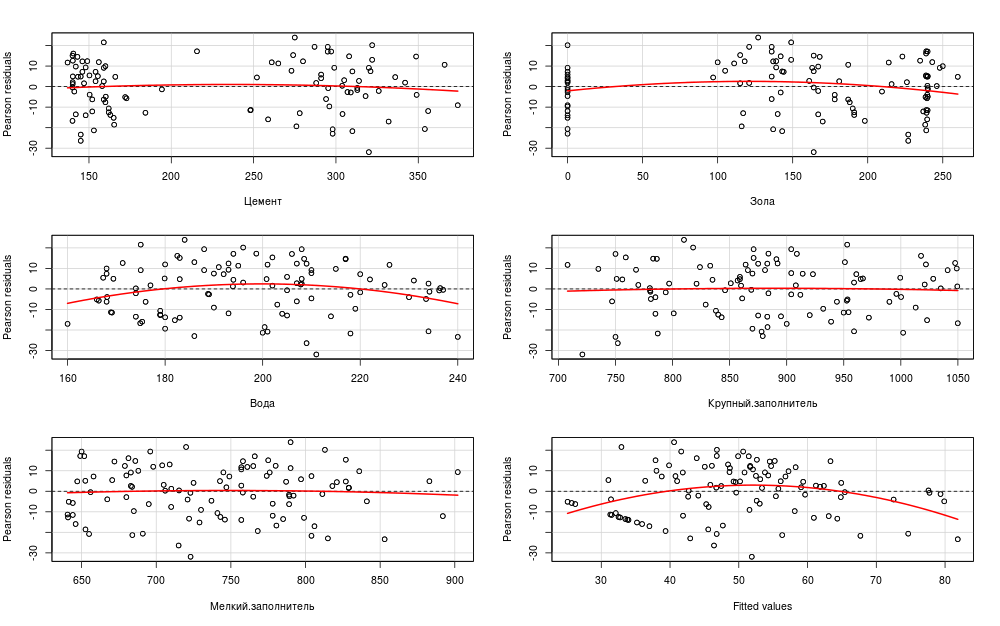
\includegraphics[scale=0.4]{resplots.png}
  \caption{Остатки для модели 2.}
\end{figure}

Критерий Фишера не показывает существенной разницы между моделями 1 и 2 ($p = 0.8283$).

\subsection{Модель 3}

Видно, что зависимости остатков для Золы и Воды имеют квадратичный характер.
Добавим квадраты этих признаков в модель.

\begin{verbatim}
> fit3 <- lm(formula = Растекание ~ Цемент + Зола + I(Зола^2) + Вода
  + I(Вода^2) + Крупный.заполнитель + Мелкий.заполнитель, data = data)
> summary(fit3)

Call:
lm(formula = Растекание ~ Цемент + Зола + 
    I(Зола^2) + Вода + I(Вода^2) + Крупный.заполнитель + 
    Мелкий.заполнитель, data = data)

Residuals:
    Min      1Q  Median      3Q     Max 
-34.079  -8.950   2.028   8.290  22.377 

Coefficients:
                      Estimate Std. Error t value Pr(>|t|)    
(Intercept)         -5.038e+02  1.370e+02  -3.678 0.000389 ***
Цемент               5.349e-02  1.940e-02   2.758 0.006978 ** 
Зола                 1.380e-01  5.125e-02   2.692 0.008391 ** 
I(Зола^2)           -2.810e-04  2.084e-04  -1.349 0.180575    
Вода                 3.141e+00  1.265e+00   2.483 0.014783 *  
I(Вода^2)           -5.962e-03  3.136e-03  -1.901 0.060354 .  
Крупный.заполнитель  8.461e-02  2.275e-02   3.720 0.000338 ***
Мелкий.заполнитель   9.301e-02  2.520e-02   3.691 0.000373 ***
---
Signif. codes:  0 ‘***’ 0.001 ‘**’ 0.01 ‘*’ 0.05 ‘.’ 0.1 ‘ ’ 1

Residual standard error: 12.43 on 95 degrees of freedom
Multiple R-squared:  0.5337,	Adjusted R-squared:  0.4994 
F-statistic: 15.54 on 7 and 95 DF,  p-value: 2.028e-13
\end{verbatim}

У полученной модели:
$$
  R^2 = 0.5337, \; R^2_{\alpha} = 0.4994, \; F = 15.54, \; \text{p-value} = 2.028 \cdot 10^{-13}
$$

\begin{tabularx}{\textwidth}{ |X|c| }
  \hline
  Критерий & p-value \\
  \hline
  Шапиро-Уилка (нормальность) & 0.01033 \\
  \hline
  Уилкоксона (несмещенность) & 0.6345 \\
  \hline
  Бройша-Пагана (гомоскедастичность) & 0.1438 \\
  \hline
\end{tabularx}

\bigskip

На рис. 5 приведены остатки для полученной модели.

\begin{figure}[h]
  \centering
  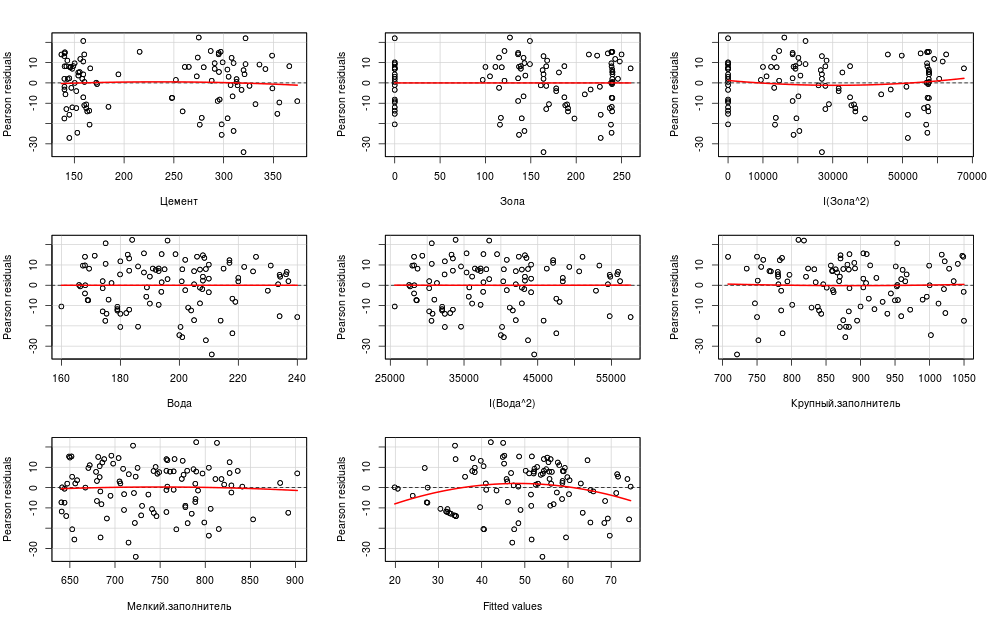
\includegraphics[scale=0.4]{resplots_3.png}
  \caption{Остатки для модели 3.}
\end{figure}

Критерий Фишера показывает превосходство модели 3 над моделью 2 ($p = 0.03707$).

\subsection{Модель 4}

Признак Зола\textasciicircum2 получается незначимым, поэтому выкинем его из модели.

\begin{verbatim}
> fit4 <- lm(formula = Растекание ~ Цемент + Зола + Вода + I(Вода^2) +
  Крупный.заполнитель + Мелкий.заполнитель, data = data)
> summary(fit4)

Call:
lm(formula = Растекание ~ Цемент + Зола + 
    Вода + I(Вода^2) + Крупный.заполнитель + 
    Мелкий.заполнитель, data = data)

Residuals:
    Min      1Q  Median      3Q     Max 
-33.697  -8.808   2.271   9.104  23.696 

Coefficients:
                      Estimate Std. Error t value Pr(>|t|)    
(Intercept)         -5.327e+02  1.358e+02  -3.921 0.000165 ***
Цемент               5.563e-02  1.941e-02   2.865 0.005116 ** 
Зола                 7.378e-02  1.910e-02   3.862 0.000204 ***
Вода                 3.488e+00  1.244e+00   2.804 0.006109 ** 
I(Вода^2)           -6.857e-03  3.078e-03  -2.228 0.028244 *  
Крупный.заполнитель  7.820e-02  2.234e-02   3.501 0.000706 ***
Мелкий.заполнитель   9.592e-02  2.522e-02   3.804 0.000250 ***
---
Signif. codes:  0 ‘***’ 0.001 ‘**’ 0.01 ‘*’ 0.05 ‘.’ 0.1 ‘ ’ 1

Residual standard error: 12.48 on 96 degrees of freedom
Multiple R-squared:  0.5248,	Adjusted R-squared:  0.4951 
F-statistic: 17.67 on 6 and 96 DF,  p-value: 1.081e-13
\end{verbatim}

У полученной модели:
$$
  R^2 = 0.5248, \; R^2_{\alpha} = 0.4951, \; F = 17.67, \; \text{p-value} = 1.081 \cdot 10^{-13}
$$

\begin{tabularx}{\textwidth}{ |X|c| }
  \hline
  Критерий & p-value \\
  \hline
  Шапиро-Уилка (нормальность) & 0.01824 \\
  \hline
  Уилкоксона (несмещенность) & 0.7064 \\
  \hline
  Бройша-Пагана (гомоскедастичность) & 0.05874 \\
  \hline
\end{tabularx}

\bigskip

На рис. 6 приведены остатки для полученной модели.

\begin{figure}[h]
  \centering
  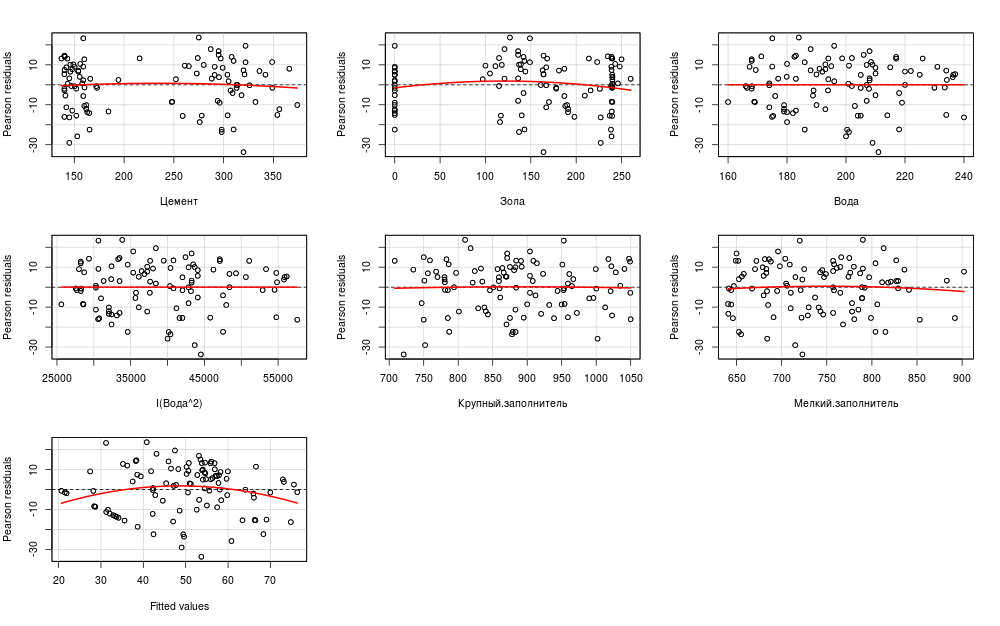
\includegraphics[scale=0.4]{resplots_4.png}
  \caption{Остатки для модели 4.}
\end{figure}

Критерий Фишера не показывает существенной разницы между моделями 3 и 4 ($p=0.1806$).

\subsection{Модель 5}

Добавим в модель попарное взаимодействие признаков и выкинем незначимые.
Получим следующую модель.

\begin{verbatim}
> fit5 <- lm(formula = Растекание ~ Зола + Вода + I(Вода^2) +
  Мелкий.заполнитель + Цемент:Зола + Зола:Крупный.заполнитель, data = data)
> summary(fit5)

Call:
lm(formula = Растекание ~ Зола + Вода + I(Вода^2) + 
    Мелкий.заполнитель + Цемент:Зола + 
    Зола:Крупный.заполнитель, data = data)

Residuals:
    Min      1Q  Median      3Q     Max 
-33.905  -8.065   0.938   8.603  24.039 

Coefficients:
                           Estimate Std. Error t value Pr(>|t|)    
(Intercept)              -4.244e+02  1.202e+02  -3.529 0.000642 ***
Зола                     -4.958e-01  1.077e-01  -4.602 1.28e-05 ***
Вода                      3.150e+00  1.180e+00   2.669 0.008940 ** 
I(Вода^2)                -5.862e-03  2.929e-03  -2.001 0.048184 *  
Мелкий.заполнитель        1.006e-01  2.300e-02   4.372 3.13e-05 ***
Зола:Цемент               3.909e-04  1.099e-04   3.557 0.000584 ***
Зола:Крупный.заполнитель  5.308e-04  1.106e-04   4.798 5.87e-06 ***
---
Signif. codes:  0 ‘***’ 0.001 ‘**’ 0.01 ‘*’ 0.05 ‘.’ 0.1 ‘ ’ 1

Residual standard error: 11.93 on 96 degrees of freedom
Multiple R-squared:  0.5662,	Adjusted R-squared:  0.5391 
F-statistic: 20.88 on 6 and 96 DF,  p-value: 1.578e-15
\end{verbatim}

У полученной модели:
$$
  R^2 = 0.5662, \; R^2_{\alpha} = 0.5391, \; F = 20.88, \; \text{p-value} = 1.578 \cdot 10^{-15}
$$

\begin{tabularx}{\textwidth}{ |X|c| }
  \hline
  Критерий & p-value \\
  \hline
  Шапиро-Уилка (нормальность) & 0.1294 \\
  \hline
  Уилкоксона (несмещенность) & 0.6966 \\
  \hline
  Бройша-Пагана (гомоскедастичность) & 0.06101 \\
  \hline
\end{tabularx}

\bigskip

На рис. 7 приведены остатки для полученной модели.

\begin{figure}[h]
  \centering
  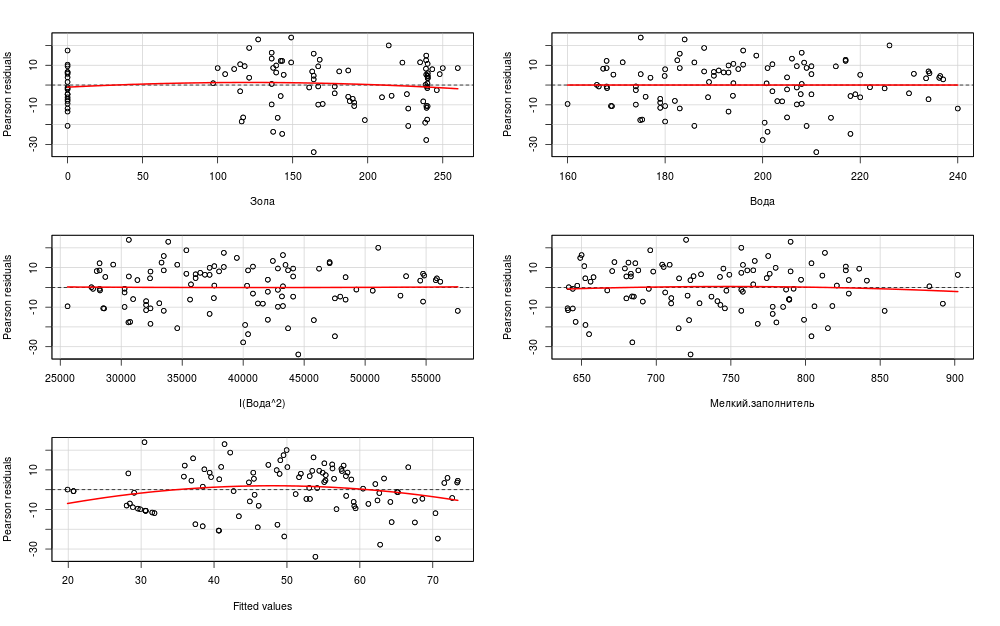
\includegraphics[scale=0.4]{resplots_5.png}
  \caption{Остатки для модели 5.}
\end{figure}

Критерий Давидсона-Маккиннона показывает превосходство модели 5 над моделью 4 ($p_1 = 0.0003, p_2 = 0.98$).

\subsection{Модель 6}

Исключим наблюдения с наибольшими расстояниями Кука (см. рис. 8) и перестроим модель 5.

\begin{figure}[h]
  \centering
  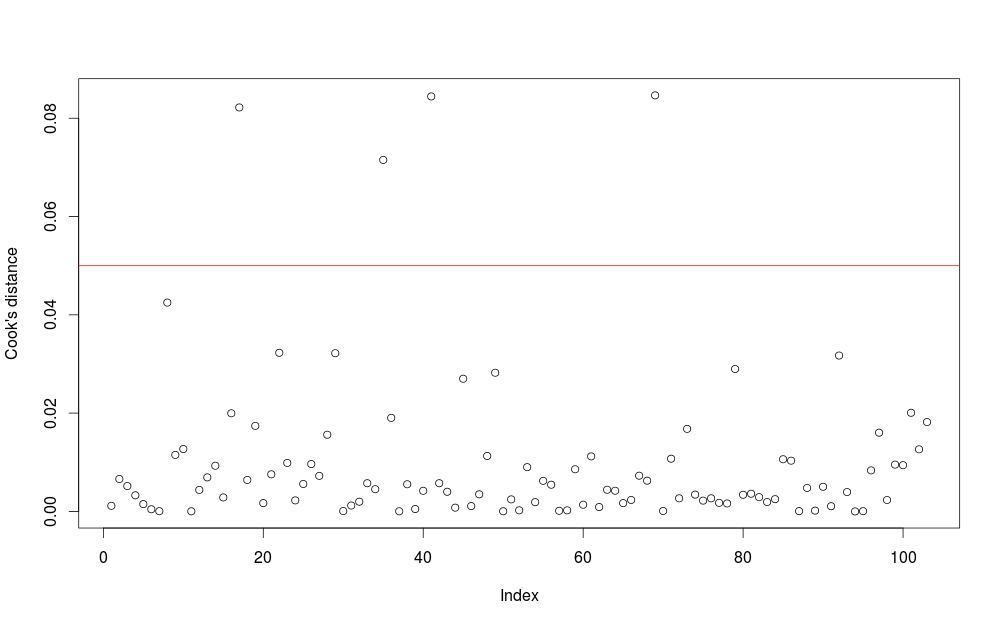
\includegraphics[scale=0.4]{cooks.png}
  \caption{Расстояния Кука для модели 5.}
\end{figure}

\begin{verbatim}
> fit6 <- lm(formula = Растекание ~ Зола + Вода + I(Вода^2) +
  Мелкий.заполнитель + Цемент:Зола + Зола:Крупный.заполнитель,
  data = data[c(-17, -35, -41, -69),])
> summary(fit6)

Call:
lm(formula = Растекание ~ Зола + Вода + I(Вода^2) + 
    Мелкий.заполнитель + Цемент:Зола + 
    Зола:Крупный.заполнитель, data = data[c(-17, 
    -35, -41, -69), ])

Residuals:
    Min      1Q  Median      3Q     Max 
-26.294  -7.235   1.738   7.362  24.138 

Coefficients:
                           Estimate Std. Error t value Pr(>|t|)    
(Intercept)              -5.240e+02  1.112e+02  -4.712 8.68e-06 ***
Зола                     -4.717e-01  1.120e-01  -4.211 5.92e-05 ***
Вода                      4.213e+00  1.094e+00   3.852 0.000216 ***
I(Вода^2)                -8.497e-03  2.714e-03  -3.131 0.002333 ** 
Мелкий.заполнитель        9.081e-02  2.160e-02   4.205 6.05e-05 ***
Зола:Цемент               3.979e-04  1.064e-04   3.740 0.000320 ***
Зола:Крупный.заполнитель  5.122e-04  1.137e-04   4.503 1.96e-05 ***
---
Signif. codes:  0 ‘***’ 0.001 ‘**’ 0.01 ‘*’ 0.05 ‘.’ 0.1 ‘ ’ 1

Residual standard error: 10.79 on 92 degrees of freedom
Multiple R-squared:  0.6316,	Adjusted R-squared:  0.6075 
F-statistic: 26.28 on 6 and 92 DF,  p-value: < 2.2e-16
\end{verbatim}

У полученной модели:
$$
  R^2 = 0.6316, \; R^2_{\alpha} = 0.6075, \; F = 26.28, \; \text{p-value} = 2.2 \cdot 10^{-16}
$$

\begin{tabularx}{\textwidth}{ |X|c| }
  \hline
  Критерий & p-value \\
  \hline
  Шапиро-Уилка (нормальность) & 0.09962 \\
  \hline
  Уилкоксона (несмещенность) & 0.7761 \\
  \hline
  Бройша-Пагана (гомоскедастичность) & 0.2837 \\
  \hline
\end{tabularx}

\bigskip

На рис. 10 приведены остатки для полученной модели.

\begin{figure}[h]
  \centering
  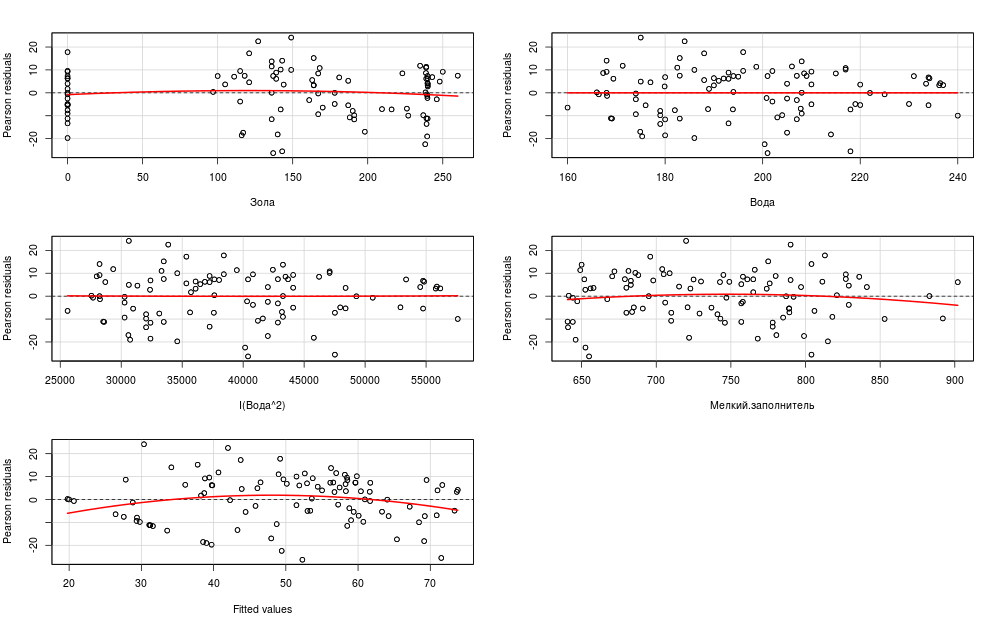
\includegraphics[scale=0.4]{resplots_6.png}
  \caption{Остатки для модели 6.}
\end{figure}

\subsection{Результат}

Итоговая модель построена по 97 из 103 исходных наблюдений и объясняет 63\% вариации логарифма отклика.

\begin{figure}[h]
  \centering
  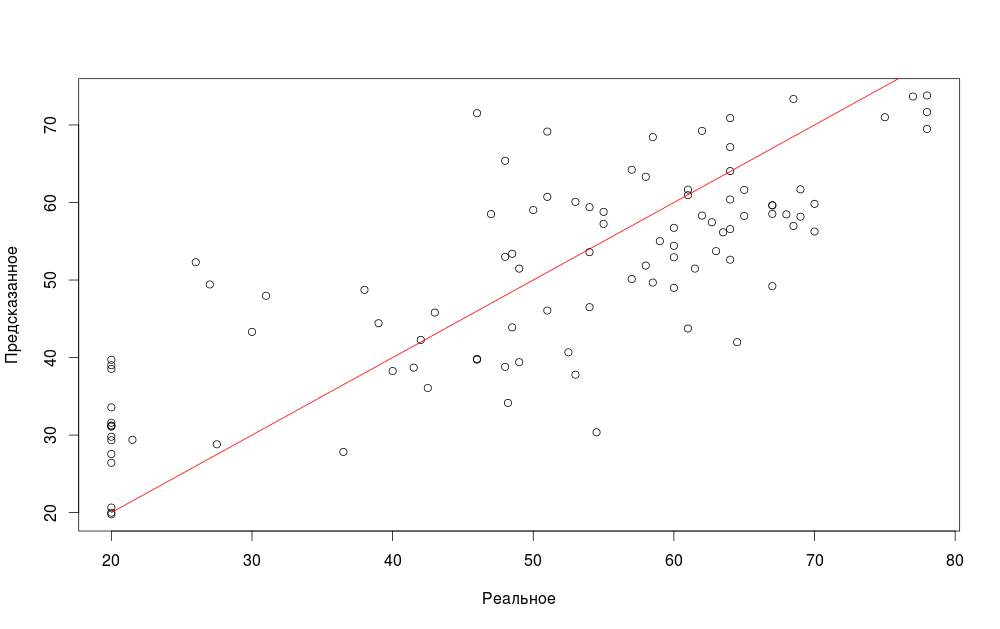
\includegraphics[scale=0.4]{result.png}
  \caption{Значения растекания для модели 6.}
\end{figure}

\section{Вывод}

Первый килограмм воды увеличивает растекание на 4.21 см (доверительный интервал (2.04, 6.39)).
Это значение уменьшается на $2 \cdot 0.008 \text{((0.003, 0.014))} \cdot \text{Вода}$ см с каждым новым килограммом воды.

Каждый килограмм мелкого заполнителя увеличивает растекание на 0.091 см (доверительный интервал (0.048, 0.133)).

Каждый килограмм золы уменьшает растекание на 0.47 см (доверительный интервал (0.25, 0.69)).
Это значение уменьшается на 0.00040 см (доверительный интервал (0.00019, 0.00061)) с каждым килограммом цемента и на 0.00051 см (доверительный интервал (0.00029, 0.00074)) с каждым килограммом крупного заполнителя.

\end{document}
